\chapter{Supporting Creative Software Activities}
People love to be creative \cite{Shneiderman2002}. Software gives people the ability to produce incredible work, from illustrations to movies to visualizations. However, to allow the flexibility and control that leads to great work, creative software applications often grow bloated with tools and commands \cite{MM-gi2000}. This creates a steep learning curve: since creative activities often require combining multiple tools and commands, the gulf of execution \cite{Hutchins1985} between these tools and the user's goals can be daunting. People spend years practicing and taking formal training to master creative software like Adobe Photoshop or Autodesk Maya. The prevalence of free and subscription-based software means that casual users now have access to tools that were once only used by professionals. Anyone can make their own animations or illustrations... if they can figure out how.

People frequently seek help online from resources shared by expert users, such as tutorials, examples, video demonstrations, and discussions. Web search provides a powerful way to quickly browse and access these resources, but it is detached from the user's work. The user must determine which resource is most relevant to their situation, and adapt it to their context \cite{Ekstrand2011, Fourney2014Intertwine, Chilana2012, Lafreniere2014a}. In addition, creative work is often open-ended and features multiple paths to success, or even multiple definitions of success \cite{Shneiderman2007}. The sensemaking challenge of using help resources combined with the open-endedness of creative work can increase overheads at best, and be paralyzing at worst, preventing people from reaching their full creative potential \cite{Shneiderman2007}. 

This dissertation introduces methods for \textbf{curating existing expert help and demonstrations} and \textbf{presenting them to users in context}, with the goal of better supporting the creative process and thus enabling people to produce better work. Leveraging existing expert-made resources enables people to learn from others more easily, and placing it in context promotes serendipity and unexpected connections.

\begin{figure}[b!]
\centering
  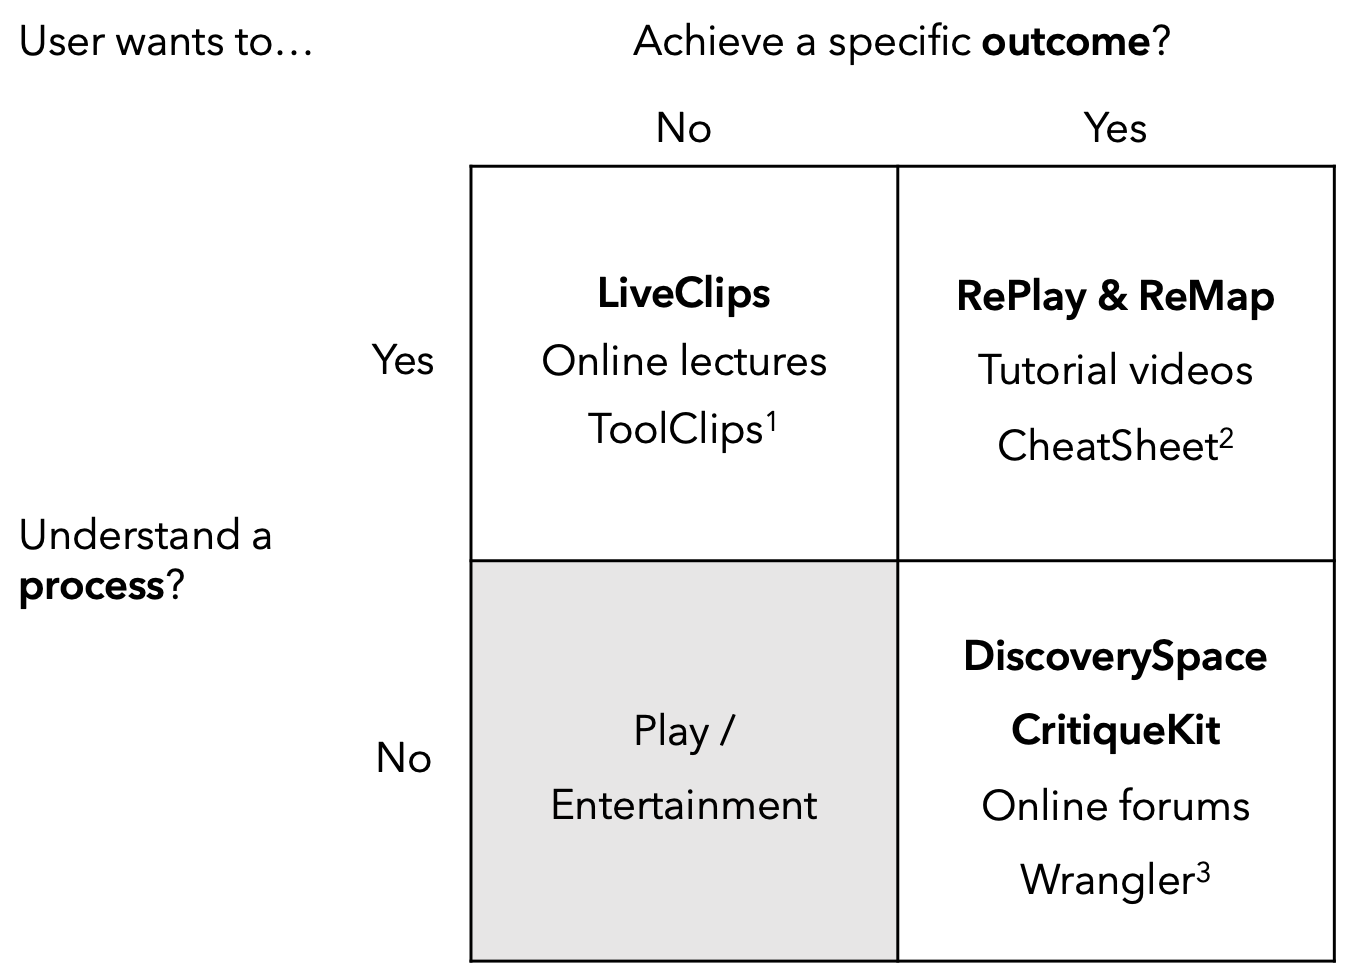
\includegraphics[width=0.7\textwidth]{figures/designspace.png}
  \caption[The interactive systems presented in this dissertation cover three of the above four quadrants depending on the goals of the user: whether they seek to understand the \textit{process} behind how something is done and/or whether they seek to accomplish a specific \textit{outcome}.]{The interactive systems presented in this dissertation cover three of the above four quadrants depending on the goals of the user: whether they seek to understand the \textit{process} behind how something is done and/or whether they seek to accomplish a specific \textit{outcome}. Bolded entries are presented in this dissertation. Non-bolded entries are examples of widely-used solutions on the web (first) and research systems that integrate with specific applications (second). \textsuperscript{1}\cite{Grossman2010a}; \textsuperscript{2}\cite{Vermette2015}; \textsuperscript{3}\cite{Kandel2011}.}~\label{fig:intro_designspace}
\end{figure}

The type of expert resource that is most helpful will differ based on whether the user wishes to understand a  \textit{process}, reach an \textit{outcome}, or both (\autoref{fig:intro_designspace}). Sometimes people are interested in understanding the process behind creative tasks, such as when learning to use a new software tool that they wish to become an expert at. Other times, people are interested only in a particular outcome, and want it done the fastest and easiest way possible. Understanding a process requires theoretical knowledge, while achieving an outcome requires practical steps \cite{Procida2017}. For example, someone seeking to become an expert InDesign user would benefit from a detailed tutorial explaining how to design a poster from scratch, while someone who needs to make a poster for an event by tomorrow might prefer using a template they can paste their event details into. A user who seeks to understand a process may or may not have a desired outcome; sometimes people follow tutorials or explore new tools in an application simply for the sake of learning the application or getting inspired, while other times they seek to learn while doing a particular task \cite{Lafreniere2013a, Procida2017}.

\begin{figure}[b!]
\centering
  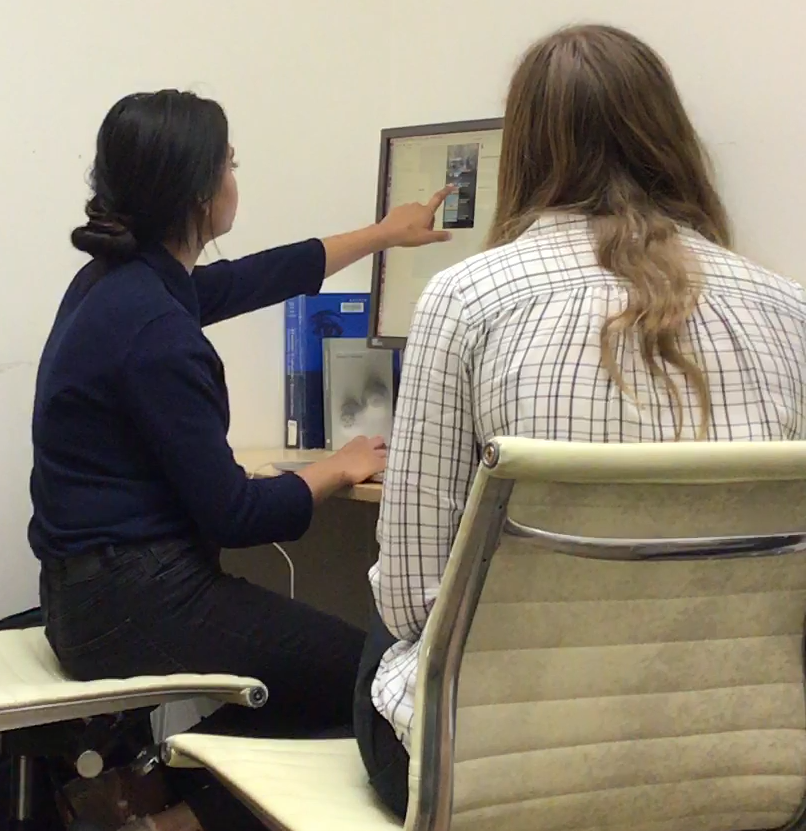
\includegraphics[width=0.35\textwidth]{figures/tutor.png}
  \hfill
  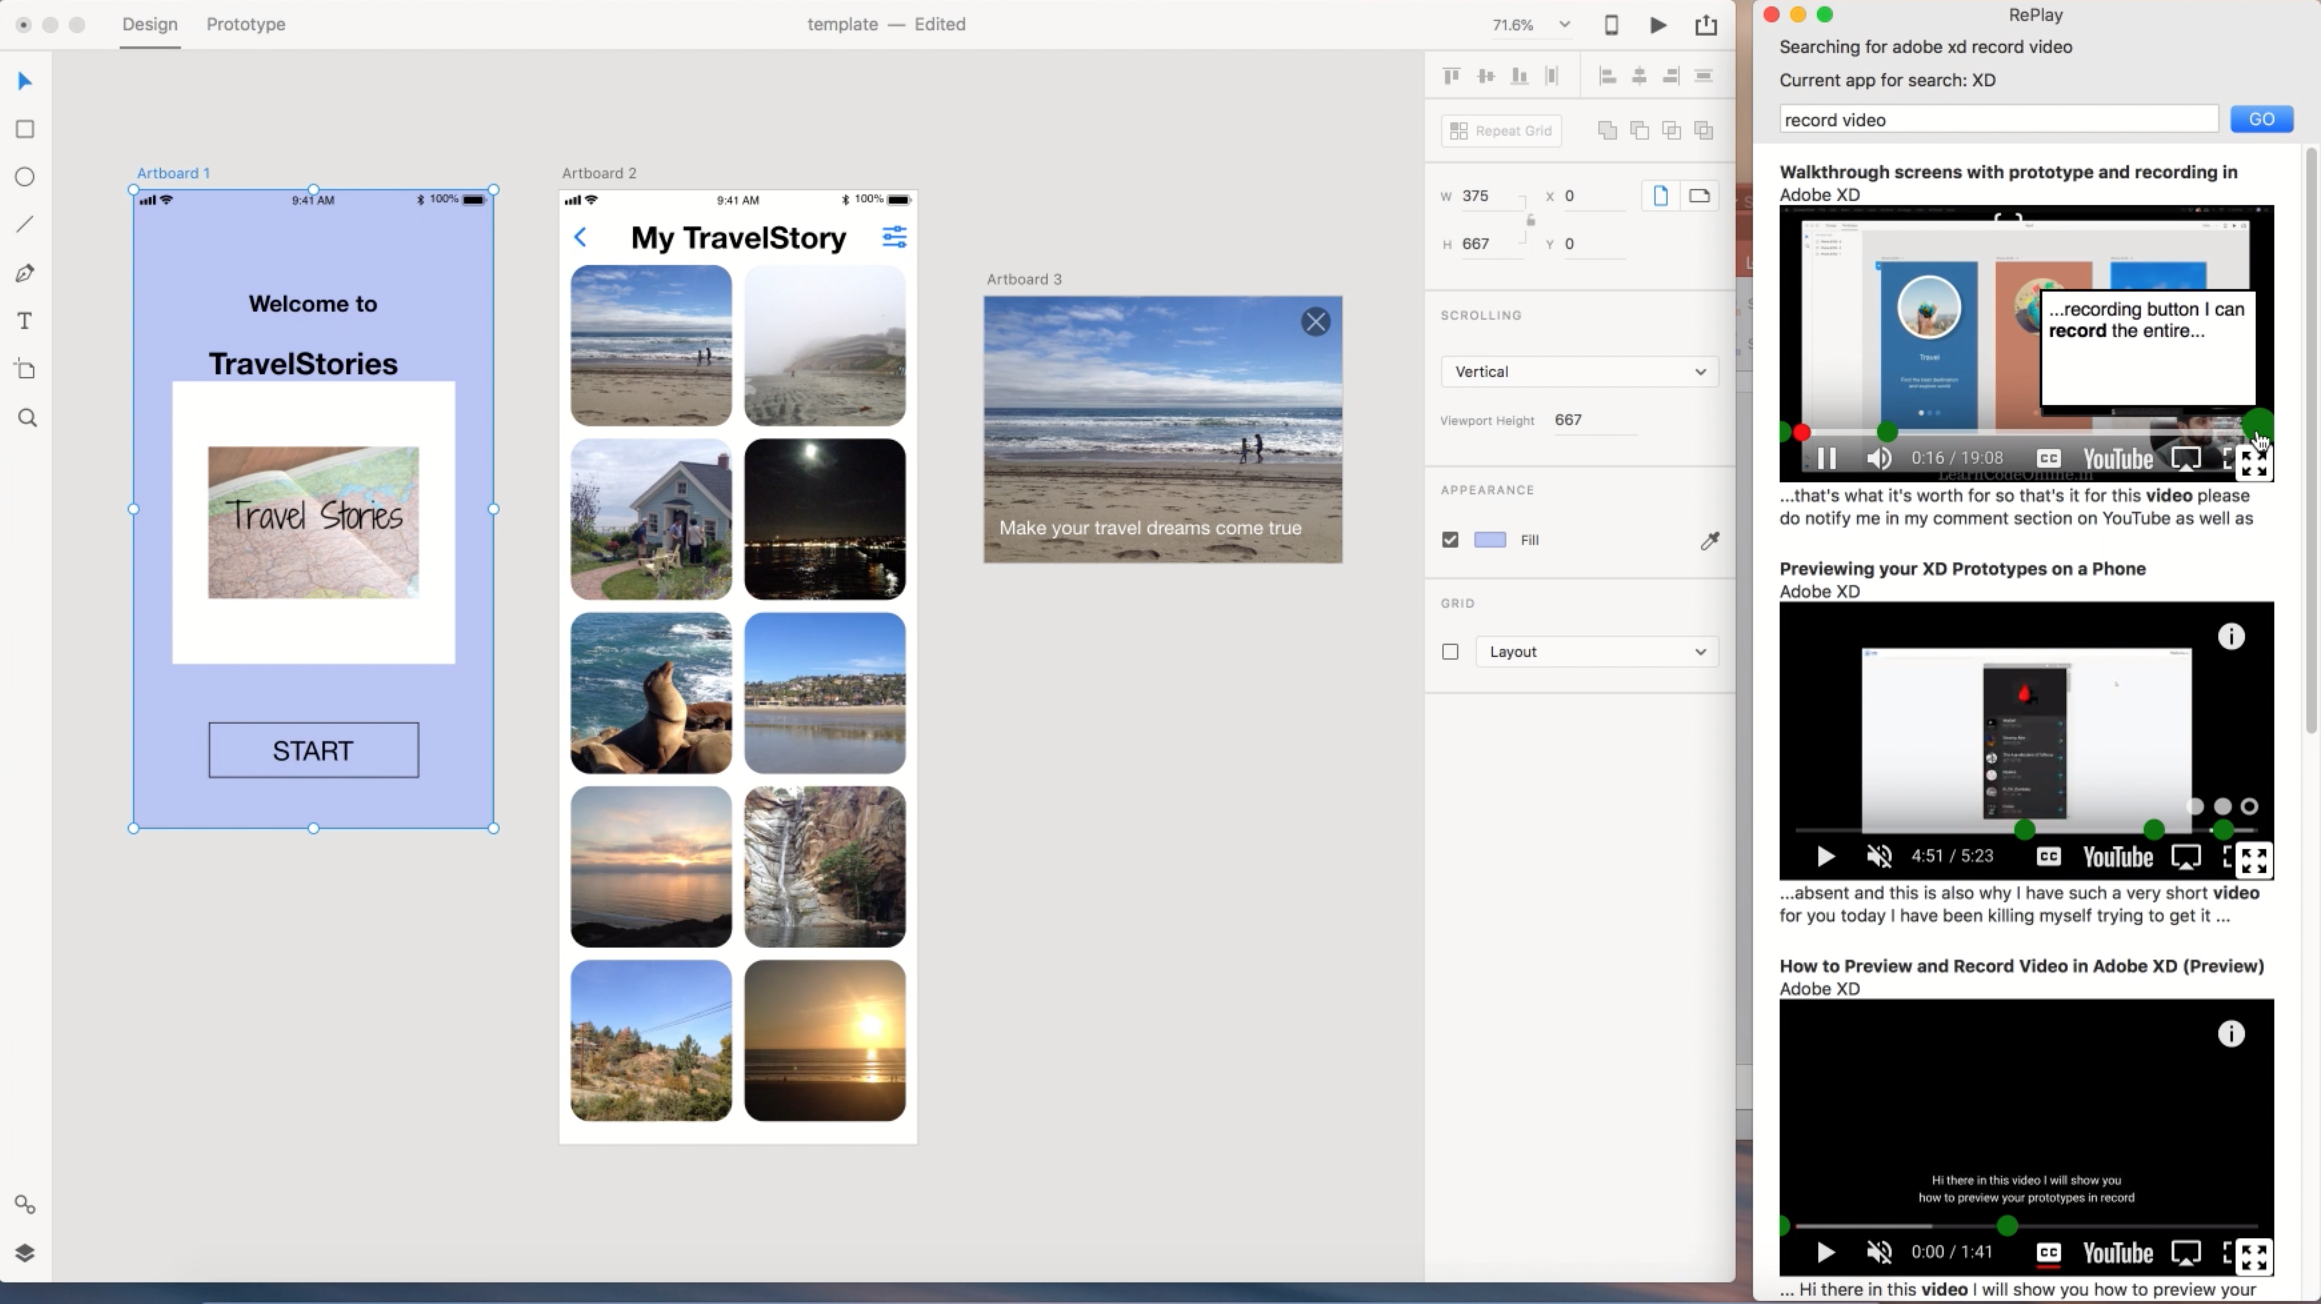
\includegraphics[width=0.64\textwidth]{figures/study.png}
  \caption{The systems presented in this dissertation aim to bring automated help one step closer to the personalized help we get from human tutors (left). For example, a screenshot from our evaluation of RePlay (right) shows a participant leveraging in-context video help to complete a creative task. }~\label{fig:intro_picture}
\end{figure}

This dissertation presents four interactive systems that explore how three different types of expert resource -- \textbf{visual media}, \textbf{executable code}, and \textbf{written text} -- can help people accomplish one or both of the above goals at a level beyond what they could have achieved otherwise (\autoref{fig:intro_designspace}). Specifically, visual media in the form of screencast videos are used to understand a process, both for achieving a specific outcome (\textit{RePlay} \& \textit{ReMap}) and for general inspiration (\textit{LiveClips}). Executable code (\textit{DiscoverySpace}) and written text (\textit{CritiqueKit}) are both used for achieving specific outcomes. Together, these systems demonstrate how expert help and demonstrations can be reused, repurposed, and curated to provide people with the resource they need, when they need it.


\section{Visual Media For Understanding Processes}
Videos are a popular learning resource for all kinds of tasks, especially creative ones \cite{Chi2012, Nguyen2015, Pongnumkul2011}. Tutorial videos that provide step-by-step instructions for a specific task are helpful for people whose goal is to learn how to do that task. Placing videos in context allows people to apply the information directly to the task at hand, promoting active learning \cite{Bonwell1991}. Other videos, such as live streams, support casual learning and inspiration by giving viewers a window into the entire, unstructured process behind a real-world project. Placing live streams in context can allow people to discover new techniques and get ideas they might not have otherwise thought of. Chapters \ref{chapter:replay}-\ref{chapter:liveclips} of this dissertation demonstrate how each of these two types of video can be curated and presented in context to support in-the-moment process understanding, with and without a specific desired outcome.

\subsection{Search and Navigation of Help Videos Supports Process and Outcome}
Tutorial videos are a popular way for creators to impart knowledge and learners to absorb it. However, videos are difficult to search, browse, and navigate, because they show a single unstructured stream of information and can typically only be explored by scrubbing on the timeline \cite{Kim2014, Pavel2015, Pavel2014}. Chapters \ref{chapter:replay}-\ref{chapter:remap} of this dissertation hypothesize that integrating search and navigation of help videos into the user's task and enhancing it with relevant context helps users achieve procedural support toward accomplishing desired outcomes. I embody this insight in the RePlay and ReMap systems for contextually presenting help videos. RePlay and ReMap gather context about the user's activity across different software applications, using it to find relevant videos. Multimodal search and contextual presentation of videos allow users to search and interact with results without taking their attention away from the task at hand. A field study ($n=7$) and lab study ($n=24$) showed that contextual video assistance helps people spend less time away from their task than web video search and replaces current video navigation strategies with more efficient workflows. An initial study with multimodal search ($n=13$) showed promise while also revealing important challenges with using speech and pointing for help-seeking.

\subsection{Recommendation of Live Stream Clips Supports Exploring Processes}
Tutorials are helpful for accomplishing specific goals, but people do not always have a particular outcome in mind when using creative software; they may not even know what outcomes are possible \cite{Matejka2009, Chaudhuri2010, ODonovan2015}. Some people watch live stream videos of artists sharing their process to get inspired and learn about new techniques (\autoref{fig:livestream_examples}). However, finding moments that are relevant and personally inspiring from these long, unstructured videos is tedious and difficult, as such moments may be few and far between. Chapter \ref{chapter:liveclips} of this dissertation hypothesizes that extracting and recommending contextually-relevant clips from creative live stream videos inside creative software promotes serendipitous discovery and inspiration throughout the creative process. I embody this insight in the LiveClips system, which automatically generates and presents clips showing demonstrations of relevant tools. Formative studies motivate this approach by exploring how people currently watch creative live streams, and what goals streamers have when making them. Initial user feedback suggests that this is a promising approach; and an online study showed that LiveClips reasonably predicts a clip's inspirational value.

\section{Code and Text For Achieving Outcomes}
Not everyone wants to learn the process behind a task; some people just want to get a task done, for which video demonstrations are too detailed. Chapters \ref{chapter:discoveryspace}-\ref{chapter:critiquekit} of this dissertation demonstrate how expert-created examples of executable code and written text can support people in exploring and achieving outcomes quickly and easily. 

\subsection{Executable Code Suggestions Enable Quick Exploration of Outcomes}
A key difficulty users often face in complex software is \textit{gulf of execution}: the gap between user intentions and the available instructions or facilities the interface provides for achieving them \cite{Hutchins1985}. Achieving a goal requires combining multiple low-level operations. This can be prohibitively difficult for novices, who are often already overwhelmed and/or uninterested in low-level details. One way to package a sequence of low-level operations into a single high-level action is to record the operations as a macro. Experts already share macros online to the user community\footnote{A Google search for ``free photoshop actions'' brings up over 39 million results, such as \href{https://www.creativebloq.com/photoshop/photoshop-actions-912784}{\nolinkurl{creativebloq.com/photoshop/photoshop-actions-912784}} and \href{https://fixthephoto.com/free-photoshop-actions}{\nolinkurl{fixthephoto.com/free-photoshop-actions}}.}; what if novices could more easily benefit from them?

Chapter \ref{chapter:discoveryspace} of this dissertation hypothesizes that integrating executable macros made by experts directly into the software streamlines their usage by reducing the steps and complexity needed to achieve advanced outcomes. I embody this insight in DiscoverySpace, a plugin for Photoshop that curates relevant photo-editing action macros shared online by the user community, and recommends relevant ones to the user for immediate use on their own photo. DiscoverySpace helps novices explore possibilities and try out advanced techniques in complex creative software. A between-subjects study ($n=28$) found that action suggestions prevent novices from losing confidence in their abilities, and help users to accomplish tasks and discover new features.

\subsection{Adaptive Suggestions of Text Examples Improve Outcomes}
Some creative tasks are complex not because of specific software, but because of the tasks themselves \cite{Brooks1987}. Providing useful feedback on creative work is one such example. Receiving useful feedback is critical for improving one's creative work, but people are rarely taught how to \textit{give} good feedback, and developing this skill takes time and practice. How might we help novice feedback givers improve the usefulness of their feedback in the moment, while they are giving it?

Chapter \ref{chapter:critiquekit} of this dissertation hypothesizes that combining examples of expert feedback with guidance that highlights their structure helps reviewers improve their feedback. I embody this insight in CritiqueKit, a system for providing feedback on creative work that incorporates suggested examples and adaptive guidance. Two real-world deployment studies ($n=37$) and two controlled experiments ($n=87$) with CritiqueKit found that adaptive suggestions combined with interactive guidance improved the quality of feedback from novice reviewers. 

\section{Thesis Statement and Contributions}
The four systems described above demonstrate how carefully curating and presenting expert help and demonstrations can support both understanding process and achieving outcomes in creative software. Together, these systems and their evaluations support my thesis statement:

\begin{quote}
    \textit{Curating expert help \& demonstrations and placing them in-context enables people to produce better work.}
\end{quote}

Each system introduces an approach for curating and ranking a different type of expert resource mined from the web (tutorial and live stream videos, executable macros, and written feedback) and a novel way to interact with these resources in-situ. Online expert help and demonstrations present a unique opportunity for creative support as they are readily available and ripe with knowledge, yet hard to find and make sense of by traditional methods. Leveraging context from the user's environment and activity provides a common ground \cite{Clark2006} for connecting users with relevant information. And finally, giving people the right resource at the right time by bringing it into their environment supports just-in-time learning and doing, enabling people to achieve outcomes that would otherwise be out of their reach. 

\subsection{Contributions}
My dissertation contributes the following:
\begin{itemize}
\item Algorithms that curate and rank four different types of expert resource (tutorial videos, live stream videos, action macros, and written feedback) based on their relevance to the user's context
\item Interfaces that present curated expert help and demonstrations in-situ for users to search, browse, navigate, and use in the context of their own work
\item Evaluations of these algorithms and interfaces that demonstrate the efficacy of contextually presenting expert resources to creative software users
\item Formative knowledge about how people currently approach creative activities and use the web for creative support
\end{itemize}

Chapter \ref{chapter:discussion} presents a discussion of the challenges that remain and open questions prompted by this research. It also discusses how the approaches presented may generalize beyond creative software tasks to other types of tasks and domains. This dissertation demonstrates the potential of bringing knowledge from user communities to everyone's fingertips, with the hope that expert help can move away from the siloed world of the web and into the creative process where everyone can benefit from it.
